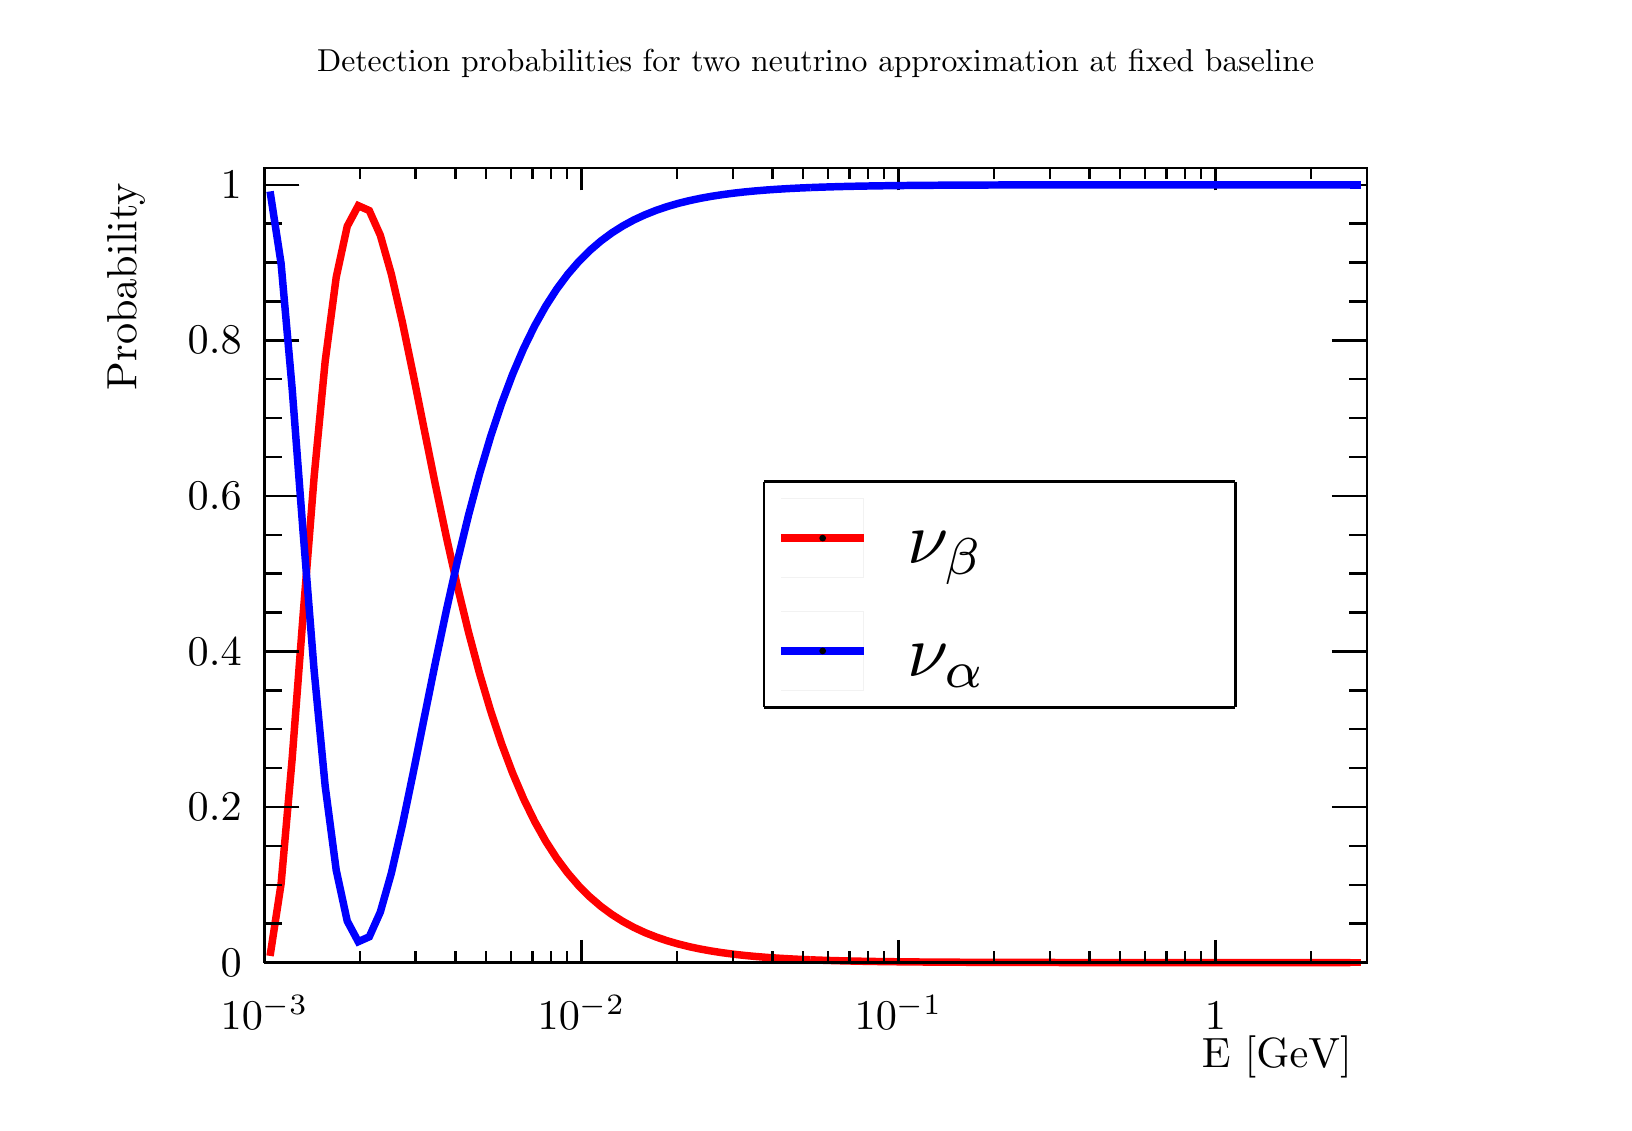
\begin{tikzpicture}
\pgfdeclareplotmark{cross} {
\pgfpathmoveto{\pgfpoint{-0.3\pgfplotmarksize}{\pgfplotmarksize}}
\pgfpathlineto{\pgfpoint{+0.3\pgfplotmarksize}{\pgfplotmarksize}}
\pgfpathlineto{\pgfpoint{+0.3\pgfplotmarksize}{0.3\pgfplotmarksize}}
\pgfpathlineto{\pgfpoint{+1\pgfplotmarksize}{0.3\pgfplotmarksize}}
\pgfpathlineto{\pgfpoint{+1\pgfplotmarksize}{-0.3\pgfplotmarksize}}
\pgfpathlineto{\pgfpoint{+0.3\pgfplotmarksize}{-0.3\pgfplotmarksize}}
\pgfpathlineto{\pgfpoint{+0.3\pgfplotmarksize}{-1.\pgfplotmarksize}}
\pgfpathlineto{\pgfpoint{-0.3\pgfplotmarksize}{-1.\pgfplotmarksize}}
\pgfpathlineto{\pgfpoint{-0.3\pgfplotmarksize}{-0.3\pgfplotmarksize}}
\pgfpathlineto{\pgfpoint{-1.\pgfplotmarksize}{-0.3\pgfplotmarksize}}
\pgfpathlineto{\pgfpoint{-1.\pgfplotmarksize}{0.3\pgfplotmarksize}}
\pgfpathlineto{\pgfpoint{-0.3\pgfplotmarksize}{0.3\pgfplotmarksize}}
\pgfpathclose
\pgfusepathqstroke
}
\pgfdeclareplotmark{cross*} {
\pgfpathmoveto{\pgfpoint{-0.3\pgfplotmarksize}{\pgfplotmarksize}}
\pgfpathlineto{\pgfpoint{+0.3\pgfplotmarksize}{\pgfplotmarksize}}
\pgfpathlineto{\pgfpoint{+0.3\pgfplotmarksize}{0.3\pgfplotmarksize}}
\pgfpathlineto{\pgfpoint{+1\pgfplotmarksize}{0.3\pgfplotmarksize}}
\pgfpathlineto{\pgfpoint{+1\pgfplotmarksize}{-0.3\pgfplotmarksize}}
\pgfpathlineto{\pgfpoint{+0.3\pgfplotmarksize}{-0.3\pgfplotmarksize}}
\pgfpathlineto{\pgfpoint{+0.3\pgfplotmarksize}{-1.\pgfplotmarksize}}
\pgfpathlineto{\pgfpoint{-0.3\pgfplotmarksize}{-1.\pgfplotmarksize}}
\pgfpathlineto{\pgfpoint{-0.3\pgfplotmarksize}{-0.3\pgfplotmarksize}}
\pgfpathlineto{\pgfpoint{-1.\pgfplotmarksize}{-0.3\pgfplotmarksize}}
\pgfpathlineto{\pgfpoint{-1.\pgfplotmarksize}{0.3\pgfplotmarksize}}
\pgfpathlineto{\pgfpoint{-0.3\pgfplotmarksize}{0.3\pgfplotmarksize}}
\pgfpathclose
\pgfusepathqfillstroke
}
\pgfdeclareplotmark{newstar} {
\pgfpathmoveto{\pgfqpoint{0pt}{\pgfplotmarksize}}
\pgfpathlineto{\pgfqpointpolar{44}{0.5\pgfplotmarksize}}
\pgfpathlineto{\pgfqpointpolar{18}{\pgfplotmarksize}}
\pgfpathlineto{\pgfqpointpolar{-20}{0.5\pgfplotmarksize}}
\pgfpathlineto{\pgfqpointpolar{-54}{\pgfplotmarksize}}
\pgfpathlineto{\pgfqpointpolar{-90}{0.5\pgfplotmarksize}}
\pgfpathlineto{\pgfqpointpolar{234}{\pgfplotmarksize}}
\pgfpathlineto{\pgfqpointpolar{198}{0.5\pgfplotmarksize}}
\pgfpathlineto{\pgfqpointpolar{162}{\pgfplotmarksize}}
\pgfpathlineto{\pgfqpointpolar{134}{0.5\pgfplotmarksize}}
\pgfpathclose
\pgfusepathqstroke
}
\pgfdeclareplotmark{newstar*} {
\pgfpathmoveto{\pgfqpoint{0pt}{\pgfplotmarksize}}
\pgfpathlineto{\pgfqpointpolar{44}{0.5\pgfplotmarksize}}
\pgfpathlineto{\pgfqpointpolar{18}{\pgfplotmarksize}}
\pgfpathlineto{\pgfqpointpolar{-20}{0.5\pgfplotmarksize}}
\pgfpathlineto{\pgfqpointpolar{-54}{\pgfplotmarksize}}
\pgfpathlineto{\pgfqpointpolar{-90}{0.5\pgfplotmarksize}}
\pgfpathlineto{\pgfqpointpolar{234}{\pgfplotmarksize}}
\pgfpathlineto{\pgfqpointpolar{198}{0.5\pgfplotmarksize}}
\pgfpathlineto{\pgfqpointpolar{162}{\pgfplotmarksize}}
\pgfpathlineto{\pgfqpointpolar{134}{0.5\pgfplotmarksize}}
\pgfpathclose
\pgfusepathqfillstroke
}
\definecolor{c}{rgb}{1,1,1};
\draw [color=c, fill=c] (0,0) rectangle (20,13.639);
\draw [color=c, fill=c] (3,1.77307) rectangle (17,11.8659);
\definecolor{c}{rgb}{0,0,0};
\draw [c,line width=0.9] (3,1.77307) -- (3,11.8659) -- (17,11.8659) -- (17,1.77307) -- (3,1.77307);
\definecolor{c}{rgb}{1,1,1};
\draw [color=c, fill=c] (3,1.77307) rectangle (17,11.8659);
\definecolor{c}{rgb}{0,0,0};
\draw [c,line width=0.9] (3,1.77307) -- (3,11.8659) -- (17,11.8659) -- (17,1.77307) -- (3,1.77307);
\definecolor{c}{rgb}{1,0,0};
\draw [c,line width=2.7] (3.0714,1.85719) -- (3.2114,2.77274) -- (3.3514,4.35643) -- (3.4914,6.19146) -- (3.6314,7.94729) -- (3.7714,9.41047) -- (3.9114,10.4764) -- (4.0514,11.1237) -- (4.1914,11.3853) -- (4.3314,11.323) -- (4.4714,11.0096) --
 (4.6114,10.5161) -- (4.7514,9.90575) -- (4.8914,9.23073) -- (5.0314,8.5317) -- (5.1714,7.8387) -- (5.3114,7.17268) -- (5.4514,6.54723) -- (5.5914,5.97024) -- (5.7314,5.44534) -- (5.8714,4.97313) -- (6.0114,4.55215) -- (6.1514,4.17961) --
 (6.2914,3.85194) -- (6.4314,3.56517) -- (6.5714,3.31526) -- (6.7114,3.09822) -- (6.8514,2.9103) -- (6.9914,2.74798) -- (7.1314,2.60806) -- (7.2714,2.48767) -- (7.4114,2.38424) -- (7.5514,2.29548) -- (7.6914,2.2194) -- (7.8314,2.15425) --
 (7.9714,2.09849) -- (8.1114,2.05081) -- (8.2514,2.01005) -- (8.3914,1.97524) -- (8.5314,1.9455) -- (8.6714,1.92012) -- (8.8114,1.89845) -- (8.9514,1.87997) -- (9.0914,1.8642) -- (9.2314,1.85075) -- (9.3714,1.83929) -- (9.5114,1.82951) --
 (9.6514,1.82117) -- (9.7914,1.81406) -- (9.9314,1.808);
\draw [c,line width=2.7] (9.9314,1.808) -- (10.0714,1.80284) -- (10.2114,1.79844) -- (10.3514,1.79469) -- (10.4914,1.79149) -- (10.6314,1.78876) -- (10.7714,1.78644) -- (10.9114,1.78446) -- (11.0514,1.78278) -- (11.1914,1.78134) -- (11.3314,1.78012)
 -- (11.4714,1.77907) -- (11.6114,1.77819) -- (11.7514,1.77743) -- (11.8914,1.77678) -- (12.0314,1.77623) -- (12.1714,1.77576) -- (12.3114,1.77536) -- (12.4514,1.77502) -- (12.5914,1.77473) -- (12.7314,1.77449) -- (12.8714,1.77428) --
 (13.0114,1.7741) -- (13.1514,1.77307) -- (13.2914,1.77307) -- (13.4314,1.77307) -- (13.5714,1.77307) -- (13.7114,1.77307) -- (13.8514,1.77307) -- (13.9914,1.77307) -- (14.1314,1.77307) -- (14.2714,1.77307) -- (14.4114,1.77307) -- (14.5514,1.77307)
 -- (14.6914,1.77307) -- (14.8314,1.77307) -- (14.9714,1.77307) -- (15.1114,1.77307) -- (15.2514,1.77307) -- (15.3914,1.77307) -- (15.5314,1.77307) -- (15.6714,1.77307) -- (15.8114,1.77307) -- (15.9514,1.77307) -- (16.0914,1.77307) --
 (16.2314,1.77307) -- (16.3714,1.77307) -- (16.5114,1.77307) -- (16.6514,1.77307) -- (16.7914,1.77307);
\draw [c,line width=2.7] (16.7914,1.77307) -- (16.9314,1.77307);
\definecolor{c}{rgb}{0,0,0};
\draw [c,line width=0.9] (3,1.77307) -- (17,1.77307);
\draw [c,line width=0.9] (3,2.05948) -- (3,1.77307);
\draw [anchor=base] (3,0.92063) node[scale=1.52731, color=c, rotate=0]{$10^{-3}$};
\draw [c,line width=0.9] (4.21205,1.91628) -- (4.21205,1.77307);
\draw [c,line width=0.9] (4.92105,1.91628) -- (4.92105,1.77307);
\draw [c,line width=0.9] (5.42409,1.91628) -- (5.42409,1.77307);
\draw [c,line width=0.9] (5.81428,1.91628) -- (5.81428,1.77307);
\draw [c,line width=0.9] (6.13309,1.91628) -- (6.13309,1.77307);
\draw [c,line width=0.9] (6.40264,1.91628) -- (6.40264,1.77307);
\draw [c,line width=0.9] (6.63613,1.91628) -- (6.63613,1.77307);
\draw [c,line width=0.9] (6.84209,1.91628) -- (6.84209,1.77307);
\draw [c,line width=0.9] (7.02632,2.05948) -- (7.02632,1.77307);
\draw [anchor=base] (7.02632,0.92063) node[scale=1.52731, color=c, rotate=0]{$10^{-2}$};
\draw [c,line width=0.9] (8.23836,1.91628) -- (8.23836,1.77307);
\draw [c,line width=0.9] (8.94736,1.91628) -- (8.94736,1.77307);
\draw [c,line width=0.9] (9.45041,1.91628) -- (9.45041,1.77307);
\draw [c,line width=0.9] (9.8406,1.91628) -- (9.8406,1.77307);
\draw [c,line width=0.9] (10.1594,1.91628) -- (10.1594,1.77307);
\draw [c,line width=0.9] (10.429,1.91628) -- (10.429,1.77307);
\draw [c,line width=0.9] (10.6624,1.91628) -- (10.6624,1.77307);
\draw [c,line width=0.9] (10.8684,1.91628) -- (10.8684,1.77307);
\draw [c,line width=0.9] (11.0526,2.05948) -- (11.0526,1.77307);
\draw [anchor=base] (11.0526,0.92063) node[scale=1.52731, color=c, rotate=0]{$10^{-1}$};
\draw [c,line width=0.9] (12.2647,1.91628) -- (12.2647,1.77307);
\draw [c,line width=0.9] (12.9737,1.91628) -- (12.9737,1.77307);
\draw [c,line width=0.9] (13.4767,1.91628) -- (13.4767,1.77307);
\draw [c,line width=0.9] (13.8669,1.91628) -- (13.8669,1.77307);
\draw [c,line width=0.9] (14.1857,1.91628) -- (14.1857,1.77307);
\draw [c,line width=0.9] (14.4553,1.91628) -- (14.4553,1.77307);
\draw [c,line width=0.9] (14.6888,1.91628) -- (14.6888,1.77307);
\draw [c,line width=0.9] (14.8947,1.91628) -- (14.8947,1.77307);
\draw [c,line width=0.9] (15.079,2.05948) -- (15.079,1.77307);
\draw [anchor=base] (15.079,0.92063) node[scale=1.52731, color=c, rotate=0]{1};
\draw [c,line width=0.9] (16.291,1.91628) -- (16.291,1.77307);
\draw [anchor= east] (17,0.572837) node[scale=1.52731, color=c, rotate=0]{E [GeV]};
\draw [c,line width=0.9] (3,11.8659) -- (17,11.8659);
\draw [c,line width=0.9] (3,11.5795) -- (3,11.8659);
\draw [c,line width=0.9] (4.21205,11.7227) -- (4.21205,11.8659);
\draw [c,line width=0.9] (4.92105,11.7227) -- (4.92105,11.8659);
\draw [c,line width=0.9] (5.42409,11.7227) -- (5.42409,11.8659);
\draw [c,line width=0.9] (5.81428,11.7227) -- (5.81428,11.8659);
\draw [c,line width=0.9] (6.13309,11.7227) -- (6.13309,11.8659);
\draw [c,line width=0.9] (6.40264,11.7227) -- (6.40264,11.8659);
\draw [c,line width=0.9] (6.63613,11.7227) -- (6.63613,11.8659);
\draw [c,line width=0.9] (6.84209,11.7227) -- (6.84209,11.8659);
\draw [c,line width=0.9] (7.02632,11.5795) -- (7.02632,11.8659);
\draw [c,line width=0.9] (8.23836,11.7227) -- (8.23836,11.8659);
\draw [c,line width=0.9] (8.94736,11.7227) -- (8.94736,11.8659);
\draw [c,line width=0.9] (9.45041,11.7227) -- (9.45041,11.8659);
\draw [c,line width=0.9] (9.8406,11.7227) -- (9.8406,11.8659);
\draw [c,line width=0.9] (10.1594,11.7227) -- (10.1594,11.8659);
\draw [c,line width=0.9] (10.429,11.7227) -- (10.429,11.8659);
\draw [c,line width=0.9] (10.6624,11.7227) -- (10.6624,11.8659);
\draw [c,line width=0.9] (10.8684,11.7227) -- (10.8684,11.8659);
\draw [c,line width=0.9] (11.0526,11.5795) -- (11.0526,11.8659);
\draw [c,line width=0.9] (12.2647,11.7227) -- (12.2647,11.8659);
\draw [c,line width=0.9] (12.9737,11.7227) -- (12.9737,11.8659);
\draw [c,line width=0.9] (13.4767,11.7227) -- (13.4767,11.8659);
\draw [c,line width=0.9] (13.8669,11.7227) -- (13.8669,11.8659);
\draw [c,line width=0.9] (14.1857,11.7227) -- (14.1857,11.8659);
\draw [c,line width=0.9] (14.4553,11.7227) -- (14.4553,11.8659);
\draw [c,line width=0.9] (14.6888,11.7227) -- (14.6888,11.8659);
\draw [c,line width=0.9] (14.8947,11.7227) -- (14.8947,11.8659);
\draw [c,line width=0.9] (15.079,11.5795) -- (15.079,11.8659);
\draw [c,line width=0.9] (16.291,11.7227) -- (16.291,11.8659);
\draw [c,line width=0.9] (3,1.77307) -- (3,11.8659);
\draw [c,line width=0.9] (3.444,1.77307) -- (3,1.77307);
\draw [c,line width=0.9] (3.222,2.26693) -- (3,2.26693);
\draw [c,line width=0.9] (3.222,2.76079) -- (3,2.76079);
\draw [c,line width=0.9] (3.222,3.25465) -- (3,3.25465);
\draw [c,line width=0.9] (3.444,3.74851) -- (3,3.74851);
\draw [c,line width=0.9] (3.222,4.24237) -- (3,4.24237);
\draw [c,line width=0.9] (3.222,4.73623) -- (3,4.73623);
\draw [c,line width=0.9] (3.222,5.23009) -- (3,5.23009);
\draw [c,line width=0.9] (3.444,5.72395) -- (3,5.72395);
\draw [c,line width=0.9] (3.222,6.21782) -- (3,6.21782);
\draw [c,line width=0.9] (3.222,6.71168) -- (3,6.71168);
\draw [c,line width=0.9] (3.222,7.20554) -- (3,7.20554);
\draw [c,line width=0.9] (3.444,7.6994) -- (3,7.6994);
\draw [c,line width=0.9] (3.222,8.19326) -- (3,8.19326);
\draw [c,line width=0.9] (3.222,8.68712) -- (3,8.68712);
\draw [c,line width=0.9] (3.222,9.18098) -- (3,9.18098);
\draw [c,line width=0.9] (3.444,9.67484) -- (3,9.67484);
\draw [c,line width=0.9] (3.222,10.1687) -- (3,10.1687);
\draw [c,line width=0.9] (3.222,10.6626) -- (3,10.6626);
\draw [c,line width=0.9] (3.222,11.1564) -- (3,11.1564);
\draw [c,line width=0.9] (3.444,11.6503) -- (3,11.6503);
\draw [c,line width=0.9] (3.444,11.6503) -- (3,11.6503);
\draw [anchor= east] (2.9,1.77307) node[scale=1.52731, color=c, rotate=0]{0};
\draw [anchor= east] (2.9,3.74851) node[scale=1.52731, color=c, rotate=0]{0.2};
\draw [anchor= east] (2.9,5.72395) node[scale=1.52731, color=c, rotate=0]{0.4};
\draw [anchor= east] (2.9,7.6994) node[scale=1.52731, color=c, rotate=0]{0.6};
\draw [anchor= east] (2.9,9.67484) node[scale=1.52731, color=c, rotate=0]{0.8};
\draw [anchor= east] (2.9,11.6503) node[scale=1.52731, color=c, rotate=0]{1};
\draw [anchor= east] (1.24,11.8659) node[scale=1.52731, color=c, rotate=90]{Probability};
\draw [c,line width=0.9] (17,1.77307) -- (17,11.8659);
\draw [c,line width=0.9] (16.556,1.77307) -- (17,1.77307);
\draw [c,line width=0.9] (16.778,2.26693) -- (17,2.26693);
\draw [c,line width=0.9] (16.778,2.76079) -- (17,2.76079);
\draw [c,line width=0.9] (16.778,3.25465) -- (17,3.25465);
\draw [c,line width=0.9] (16.556,3.74851) -- (17,3.74851);
\draw [c,line width=0.9] (16.778,4.24237) -- (17,4.24237);
\draw [c,line width=0.9] (16.778,4.73623) -- (17,4.73623);
\draw [c,line width=0.9] (16.778,5.23009) -- (17,5.23009);
\draw [c,line width=0.9] (16.556,5.72395) -- (17,5.72395);
\draw [c,line width=0.9] (16.778,6.21782) -- (17,6.21782);
\draw [c,line width=0.9] (16.778,6.71168) -- (17,6.71168);
\draw [c,line width=0.9] (16.778,7.20554) -- (17,7.20554);
\draw [c,line width=0.9] (16.556,7.6994) -- (17,7.6994);
\draw [c,line width=0.9] (16.778,8.19326) -- (17,8.19326);
\draw [c,line width=0.9] (16.778,8.68712) -- (17,8.68712);
\draw [c,line width=0.9] (16.778,9.18098) -- (17,9.18098);
\draw [c,line width=0.9] (16.556,9.67484) -- (17,9.67484);
\draw [c,line width=0.9] (16.778,10.1687) -- (17,10.1687);
\draw [c,line width=0.9] (16.778,10.6626) -- (17,10.6626);
\draw [c,line width=0.9] (16.778,11.1564) -- (17,11.1564);
\draw [c,line width=0.9] (16.556,11.6503) -- (17,11.6503);
\draw [c,line width=0.9] (16.556,11.6503) -- (17,11.6503);
\definecolor{c}{rgb}{0,0,1};
\draw [c,line width=2.7] (3.0714,11.5662) -- (3.2114,10.6506) -- (3.3514,9.06693) -- (3.4914,7.2319) -- (3.6314,5.47606) -- (3.7714,4.01289) -- (3.9114,2.94696) -- (4.0514,2.29963) -- (4.1914,2.03806) -- (4.3314,2.10031) -- (4.4714,2.41379) --
 (4.6114,2.90727) -- (4.7514,3.51761) -- (4.8914,4.19262) -- (5.0314,4.89165) -- (5.1714,5.58465) -- (5.3114,6.25067) -- (5.4514,6.87612) -- (5.5914,7.45311) -- (5.7314,7.97802) -- (5.8714,8.45022) -- (6.0114,8.8712) -- (6.1514,9.24374) --
 (6.2914,9.57142) -- (6.4314,9.85818) -- (6.5714,10.1081) -- (6.7114,10.3251) -- (6.8514,10.5131) -- (6.9914,10.6754) -- (7.1314,10.8153) -- (7.2714,10.9357) -- (7.4114,11.0391) -- (7.5514,11.1279) -- (7.6914,11.204) -- (7.8314,11.2691) --
 (7.9714,11.3249) -- (8.1114,11.3725) -- (8.2514,11.4133) -- (8.3914,11.4481) -- (8.5314,11.4779) -- (8.6714,11.5032) -- (8.8114,11.5249) -- (8.9514,11.5434) -- (9.0914,11.5592) -- (9.2314,11.5726) -- (9.3714,11.5841) -- (9.5114,11.5938) --
 (9.6514,11.6022) -- (9.7914,11.6093) -- (9.9314,11.6154);
\draw [c,line width=2.7] (9.9314,11.6154) -- (10.0714,11.6205) -- (10.2114,11.6249) -- (10.3514,11.6287) -- (10.4914,11.6319) -- (10.6314,11.6346) -- (10.7714,11.6369) -- (10.9114,11.6389) -- (11.0514,11.6406) -- (11.1914,11.642) -- (11.3314,11.6432)
 -- (11.4714,11.6443) -- (11.6114,11.6452) -- (11.7514,11.6459) -- (11.8914,11.6466) -- (12.0314,11.6471) -- (12.1714,11.6476) -- (12.3114,11.648) -- (12.4514,11.6483) -- (12.5914,11.6486) -- (12.7314,11.6489) -- (12.8714,11.6491) --
 (13.0114,11.6493) -- (13.1514,11.6494) -- (13.2914,11.6495) -- (13.4314,11.6496) -- (13.5714,11.6497) -- (13.7114,11.6498) -- (13.8514,11.6499) -- (13.9914,11.65) -- (14.1314,11.65) -- (14.2714,11.65) -- (14.4114,11.6501) -- (14.5514,11.6501) --
 (14.6914,11.6501) -- (14.8314,11.6502) -- (14.9714,11.6502) -- (15.1114,11.6502) -- (15.2514,11.6502) -- (15.3914,11.6502) -- (15.5314,11.6502) -- (15.6714,11.6502) -- (15.8114,11.6502) -- (15.9514,11.6503) -- (16.0914,11.6503) -- (16.2314,11.6503)
 -- (16.3714,11.6503) -- (16.5114,11.6503) -- (16.6514,11.6503) -- (16.7914,11.6503);
\draw [c,line width=2.7] (16.7914,11.6503) -- (16.9314,11.6503);
\definecolor{c}{rgb}{1,1,1};
\draw [color=c, fill=c] (2,12.8206) rectangle (18,13.5708);
\definecolor{c}{rgb}{0,0,0};
\draw (10,13.1957) node[scale=1.14549, color=c, rotate=0]{Detection probabilities for two neutrino approximation at fixed baseline};
\definecolor{c}{rgb}{1,1,1};
\draw [color=c, fill=c] (9.34097,5.01433) rectangle (15.3295,7.87966);
\definecolor{c}{rgb}{0,0,0};
\draw [c,line width=0.9] (9.34097,5.01433) -- (15.3295,5.01433);
\draw [c,line width=0.9] (15.3295,5.01433) -- (15.3295,7.87966);
\draw [c,line width=0.9] (15.3295,7.87966) -- (9.34097,7.87966);
\draw [c,line width=0.9] (9.34097,7.87966) -- (9.34097,5.01433);
\draw [anchor=base west] (10.8381,6.84097) node[scale=2.6728, color=c, rotate=0]{$\nu_{\beta}$};
\definecolor{c}{rgb}{0.95,0.95,0.95};
\draw [c] (9.56554,6.66189) -- (10.6135,6.66189) -- (10.6135,7.66476) -- (9.56554,7.66476);
\definecolor{c}{rgb}{1,0,0};
\draw [c,line width=2.7] (9.56554,7.16332) -- (10.6135,7.16332);
\definecolor{c}{rgb}{0,0,0};
\foreach \P in {(10.0895,7.16332)}{\draw[mark options={color=c,fill=c},mark size=2.402402pt,mark=*,mark size=1pt] plot coordinates {\P};}
\draw [anchor=base west] (10.8381,5.40831) node[scale=2.6728, color=c, rotate=0]{$\nu_{\alpha}$};
\definecolor{c}{rgb}{0.95,0.95,0.95};
\draw [c] (9.56554,5.22923) -- (10.6135,5.22923) -- (10.6135,6.23209) -- (9.56554,6.23209);
\definecolor{c}{rgb}{0,0,1};
\draw [c,line width=2.7] (9.56554,5.73066) -- (10.6135,5.73066);
\definecolor{c}{rgb}{0,0,0};
\foreach \P in {(10.0895,5.73066)}{\draw[mark options={color=c,fill=c},mark size=2.402402pt,mark=*,mark size=1pt] plot coordinates {\P};}
\end{tikzpicture}
